% This is the template for submission of abstracts to NetSci 2017 in Indianapolis, IN.
% It is modified from NetSci 2016.
% The editor of the booklet reserves the right to modify your submission.

%% To process this file run LaTeX2e

%%********DO NOT EDIT****************
\documentclass[11pt]{article}
\usepackage{mathptmx}
\usepackage{graphicx}
\pagestyle{empty}

\setlength\topmargin{0pt}
\addtolength\topmargin{-\headheight}
\addtolength\topmargin{-\headsep}
\setlength\oddsidemargin{0pt}
\setlength\textwidth{\paperwidth}
\addtolength\textwidth{-2in}
\setlength\textheight{\paperheight}
\addtolength\textheight{-2in}
\usepackage{layout}

\renewcommand{\title}[1]{\noindent\textbf{#1}\bigskip\\}
\renewcommand{\author}[1]{\noindent #1\bigskip\\}
%%***********************************

\begin{document}

%**********USER DEFINED**************
%Enter title here
\title{Phases of Physical 3D Networks}
%Enter author(s) and address here
%Enter abstract here
\author{Nima Dehmamy,$^1$ Soodabeh Milanlouei,$^1$ Albert-L\'aszl\'o Barab\'asi$^1$\bigskip\\
{\small
1. Northeastern University, Boston, MA, USA
}
} %author
\date{\today}

\begin{abstract}
Analyzing networks embedded in 3D space is crucial for understanding brain anatomy and pathologies pertaining to physical connections in the brain. 
Devising physical 3D layouts for networks is also of interest for  visualization purposes.
Additionally, given the recent advancements in 3D printing technology, 3D layouts may have practical value in design and manufacturing of complex devices. 
It is important to have efficient and economical 3D layout algorithm for networks. 
The role of network topology in layouts and the limitations it imposes on the feasibility of layouts must, thus, be studied.
We develop a minimal 3D layout algorithm for networks, inspired by force-directed layouts. 
We analyze the spatial properties of our layouts and find two phases based on link thickness and derive the phase transition criterion.  
In both phases, different network topologies turn out to be very similar in their volumetric properties and are not distinguishable based on volume. 
Relative link orientation, does differentiate the topologies when links are thin, but fails to do so at large link thickness. 
Thus, we discover a universal phase for 3D networks when link thickness is large.
Comparing against brain literature, we find that many mammalian brains may be related to this universal phase at the level of connections between large brain regions.  
We also argue that primate brains most likely do not belong to this universal phase. 
\end{abstract}

% \bigskip
% \noindent[1] You may add a reference.
% \\
% \noindent[2] You may add a reference.
% \\
% \noindent[3] You may add a reference.
% \\


\begin{figure}[!h]
    \centering
    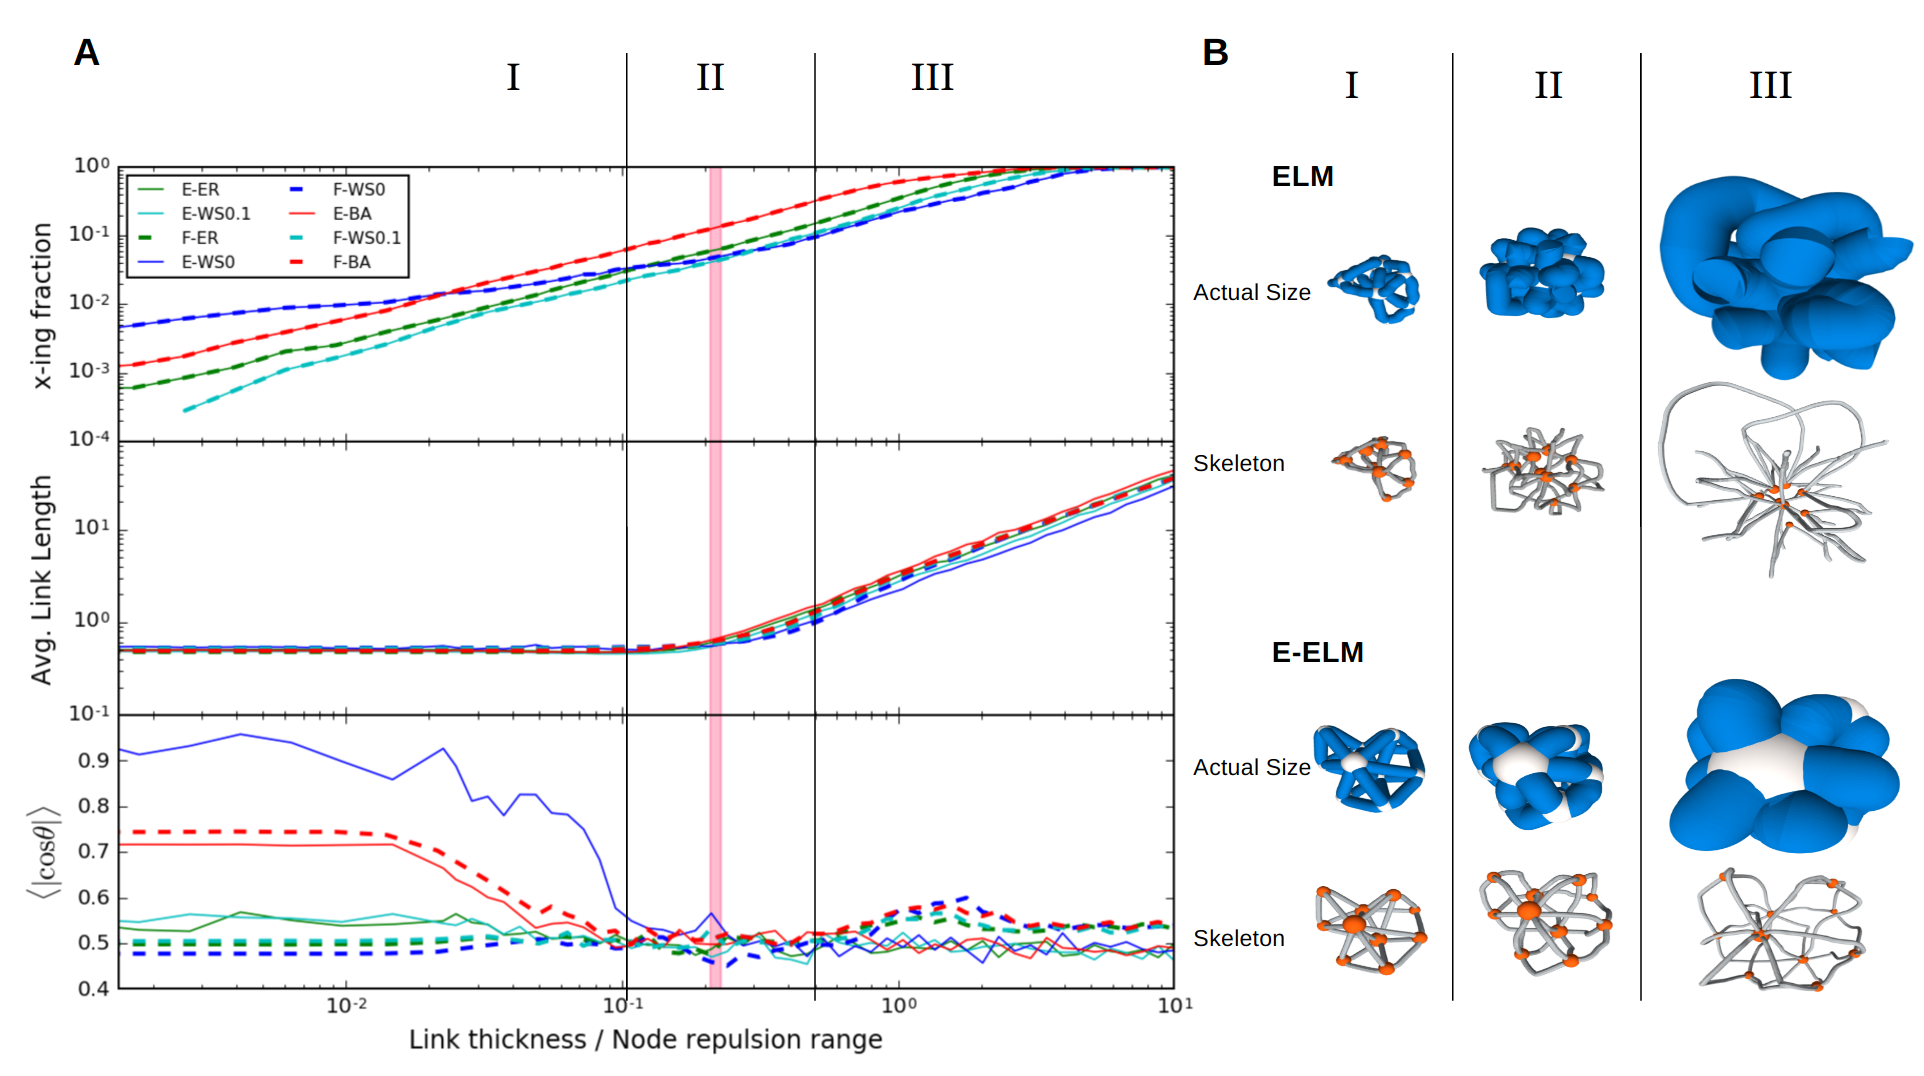
\includegraphics[width=.8\columnwidth]{fig-09-19/phase-compare-4.png}
    \caption{\small { \bf Phases of the Elastic Link Model (ELM) vs. Emancipated ELM (E-ELM):} Right: Examples of layout in each of the three regions of the diagrams on the left (blue links: actual thickness; gray links: skeleton showing paths).
    Left: Fraction of crossing links, average link length and average relative angle of adjacent link segments $\langle|\cos\theta |\rangle$. 
    Dashed lines are ELM (prefix ``F-'' in legend), solids are E-ELM (prefix ``E-''). 
    Each color signifies a network topology: ER: Erd\"os-Renyi; BA: Barabasi-Albert; WS0: Watts-Strogatz with no rewiring; WS0.1: WS with $p=0.1$ rewiring. 
    % The average link length (second plot) is not a good discriminant of different network topologies. Neither does it distinguish between ELM and E-ELM. 
    % The $\be{|\cos\theta |}$, on the other hand, does discriminate between both topology and the two layouts ELM and E-ELM in region \RNum{1}, which we call the ``slim phase''. 
    % In the transition region, \RNum{2}, and the ``hair-ball phase'', \RNum{3}, however, different topologies laid out using ELM are indistinguishable. 
    % Similarly the hair-ball phase cannot distinguish topologies in E-ELM. 
    }
    \label{fig:phase-compare}
\end{figure}


% Place the abstract of your talk/poster here, 250 Words maximum.
% Mathematical formulae may be set in LaTeX, but do NOT use the
% bibliography environment -- if you must have references, use an 
% enumerated list.
%
% Your abstract (plus one figure) should not exceed one page.
%
% Check carefully.

%************************************
\end{document}